The details of the metrics selected for quantitative evaluations and that these metrics will be applied on codebases using the CodeMR static code analysis tool are mentioned in section \ref{section:3.2}. However, the information that would facilitate the interpretation of the charts and reports produced by CodeMR was not shared. It is deemed appropriate to share this information in this section so that the results can be understood and interpreted more easily.

CodeMR tool firstly performs value calculations for each metric over the provided code base and presents these values. Information about the formulas used in calculating metric values and how the values are interpreted can be accessed through the CodeMR documentation\footnote{\label{fn:codemr} \url{https://www.codemr.co.uk/documents/}}. The figure below is an example of how these values are presented. These values were calculated with the help of the CodeMR Intellij IDEA plugin.
\begin{figure}[ht!]
    \centering
    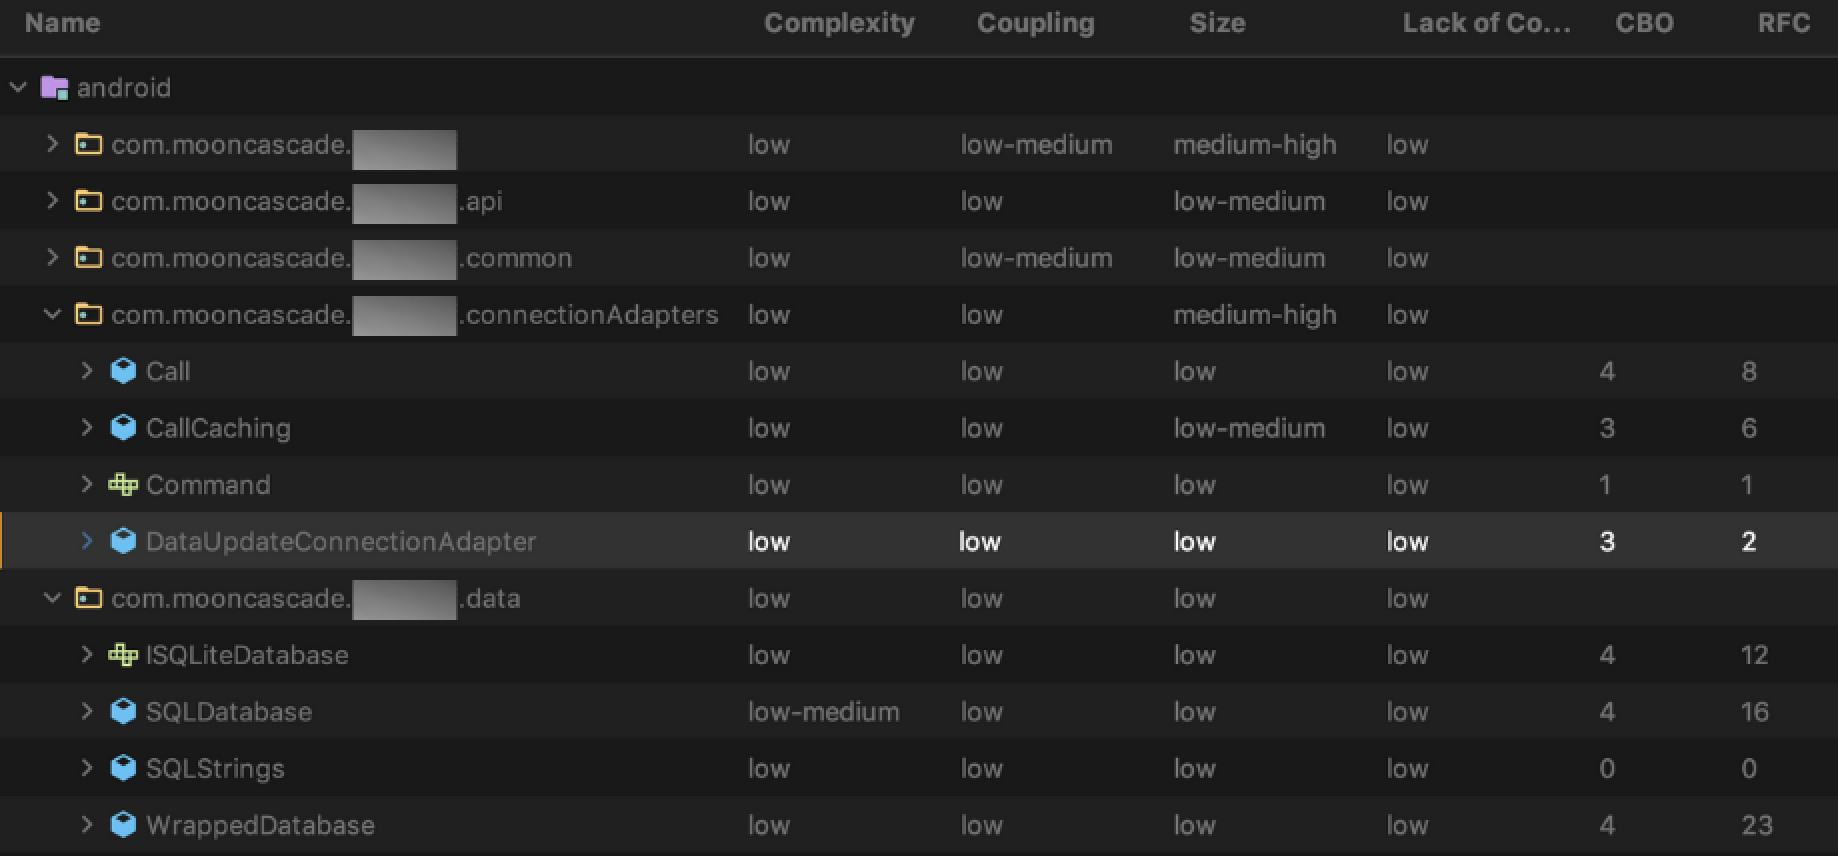
\includegraphics[scale=0.34]{figures/code-mr-metric-val.png}
    \caption{CodeMR Metric Value Presentation}
    \label{fig:code-mr-metric-val}
\end{figure}
\FloatBarrier
As shown in Fig \ref{fig:code-mr-metric-val}, the tool calculates each metric it offers and presents its results. Values for each metric are presented at project, module, package and class scopes. However, in the evaluations within the scope of this study, only the results of the metrics previously determined and explained in section \ref{section:3.2} were used.

The CodeMR tool uses different visualization methods in the reports generated by the application of metrics. The charts are created with the help of these different visualization techniques based on the metric values whose details are shared above. Within this study's scope, the visualization methods known as "Metric Distribution" and "Package Structure" in CodeMR literature were preferred to present the results of the evaluations. The main reason for choosing this methods is that it makes the visual understanding of the results easier than other methods and also these methods provide a better situational perceptibility for projects. These visualization techniques were used to visualize the data obtained as a result of applying the metrics specified in section 3.2 and the analysis presented by CodeMR on complexity, coupling and cohesion concepts. Other visualization methods and charts are very detailed, and sharing such detailed results is beyond this study's scope. 

There are two important points to be aware of when interpreting the charts created by these methods using CodeMR. The first of these points is legends used to indicate metric levels. As can be seeń in Fig. \ref{fig:code-mr-legends}, each colour corresponds to a metric level that is represented by a certain metric value threshold. The second important point is how the percentages on these charts are calculated while realizing the charts created by CodeMR. There might be different metric levels in different percentages in the charts. These percentages of metric levels for the selected metrics are illustrated in charts proportionally to the code size of classes in this level.
\begin{figure}[ht!]
    \centering
    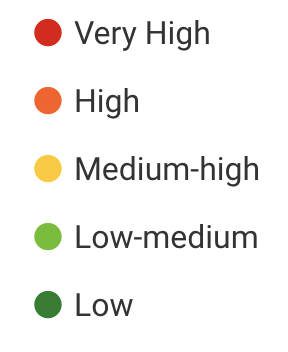
\includegraphics[scale=0.7]{figures/code-mr-legends.png}
    \caption{CodeMR Metric Level Indicators}
    \label{fig:code-mr-legends}
\end{figure}
\FloatBarrier

 %A similar situation applies to the "Package Structure" method. Package structure displays project’s packages and encapsulated classes in a hierarchical way with a circle pack layout. The size of each circle is proportional to the size of the represented class/package, and the colour of each circle represents the level for the selected metric. Below is a chart created by CodeMR using the "Package Structure" method and the "C3" sample metric.
%\begin{figure}[ht!]
 %   \centering
  %  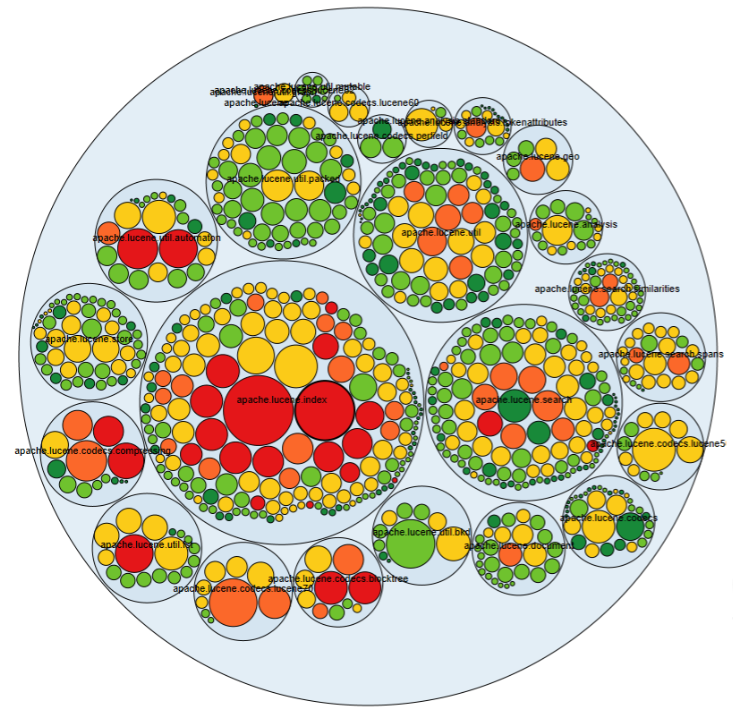
\includegraphics[scale=0.5]{figures/code-mr-package-structure.png}
   % \caption{Sample CodeMR Package Structure Chart}
    %\label{fig:code-mr-package-structure}
%\end{figure}
%\FloatBarrier

As explained above, these two points are essential when interpreting the charts that are shared in the next three sections. The details of the metrics and their thresholds ,visualization methods and, charts used can be found in the CodeMR documentation $^{\ref{fn:codemr}}$.

